\documentclass[a4paper,12pt]{article}
%\documentclass[fleqn]{article}

% ---パッケージ---
\usepackage{amsmath,amssymb}    %数式用
\usepackage{tcolorbox}   %囲み枠用(tcolorboxに変更)
\usepackage{geometry}   %余白調節
\usepackage{tikz}  % ← 図を描くためのTikZパッケージ
\geometry{margin=25mm}  %余白を少し狭く
\usetikzlibrary{decorations.pathmorphing,patterns,positioning,arrows.meta} % バネ・壁の模様
\tikzset{
  block/.style = {draw, rectangle, minimum height=2em, minimum width=3em},
  sum/.style = {draw, circle, inner sep=0pt, minimum size=5mm},
  input/.style = {coordinate},
  output/.style = {coordinate}
}
\usetikzlibrary{calc}
\usepackage{pgfplots}  % ← 追加(グラフ用)
\pgfplotsset{compat=newest} % ← 推奨設定

% --- 日本語用パッケージ ---
\usepackage{luatexja}         % 日本語表示に必要
\usepackage{luatexja-fontspec} % フォント指定用

% --- フォント指定(Overleaf標準フォント)---
\setmainjfont{IPAexMincho}  % 明朝体
%\setmainjfont{IPAexGothic}  % ゴシック体にしたい場合

% --- tcolorbox の設定 ---
\tcbset{
    colframe=black,
    colback=white,         % 本文の背景(白)
    boxrule=0.8pt,
    arc=3pt,
    outer arc=3pt,
    boxsep=4pt,
    coltitle=black,
    colbacktitle=gray!20,  % タイトルの背景(グレー)
    fonttitle=\normalsize
}

\begin{document}

\noindent
\text{制御工学Ⅰ 演習② 解答}

\vspace{10mm}


% ---------------[1]--------------- 済
\noindent
1. 次の伝達関数で表されるシステムのラプラス逆変換を行え。
\vspace{-4mm}
\[
\renewcommand{\arraystretch}{3.0} % ← 行の高さ倍率を変更(1.0が標準)
\begin{tabular}{@{}rl@{\quad\quad}rl@{}}
(1) & $G_1(s) = \dfrac{1}{s^2+2s+2}$                 & (2) & $G_2(s) = \dfrac{6}{s^3+6s^2+11s+6}$ \\
\end{tabular}
\]

\begin{tcolorbox}[title={1. (1) \(G_1(s) = \dfrac{1}{s^2+2s+2}\) }]
  \vspace{-3mm}
    \begin{align*}
    &\quad G_1(s) =\frac{ 1 }{ s^2 + 2s + 2}  \\
    &\Leftrightarrow G_1(s) =\frac{ 1 }{ ( s + 1 )^2+ 1^2} \\
    &\Leftrightarrow G_1(s) 
    = \frac{ 1}{ ( s + 1 )^2+ 1^2}
\end{align*}

\quad 両辺にラプラス逆変換を施すと,

\vspace{-3mm}
\begin{align*}
    &\qquad \mathcal{L}^{-1} \left[ G_1(s) \right] 
    =\mathcal{L}^{-1} \left[ \frac{ 1 }{ ( s + 1 )^2+ 1^2} \right]\\
    &\Leftrightarrow g_1(t) = e^{-t} sin(t)
\end{align*}
\end{tcolorbox}

\begin{tcolorbox}[title={1. (2) \(G_2(s) = \dfrac{6}{s^3+6s^2+11s+6}\) }]
  \vspace{-3mm}
\begin{align*}
    &\qquad X(s) =\frac{ 1 }{ s^3 +6 s^2+ 11s + 6 }  \\
    &\Leftrightarrow X(s) =\frac{ 1 }{ (s+1)(s+2)(s+3) }  \\
    &\Leftrightarrow X(s) 
    = \frac{(\frac{1}{2})}{s+1}
    + \frac{-1}{s + 2}
    + \frac{(\frac{1}{2})}{s + 3}
\end{align*}

\quad 両辺にラプラス逆変換を施すと,
\vspace{-3mm}
\begin{align*}
    &\qquad \mathcal{L}^{-1} \left[ X(s) \right] 
    =\mathcal{L}^{-1} \left[ \frac{(\frac{1}{2})}{s+1} \right]
    +\mathcal{L}^{-1} \left[ \frac{-1}{s + 2} \right]
    +\mathcal{L}^{-1} \left[ \frac{(\frac{1}{2})}{s + 3} \right] \\
    &\Leftrightarrow x(t) = (\frac{1}{2})e^{-t} - e^{-2t} + (\frac{1}{2})e^{-3t}
\end{align*}
\end{tcolorbox}

\newpage

% ---------------[2]---------------
\noindent
2.下図に示すシステムにおいて、システム全体の伝達関数を求めよ。なお、各伝達関数
\(G_i(s)\)については問1.の伝達関数を代入しないこと。
\vspace{2mm}

\begin{minipage}[t]{0.45\linewidth}
  (1)
  \begin{center}
    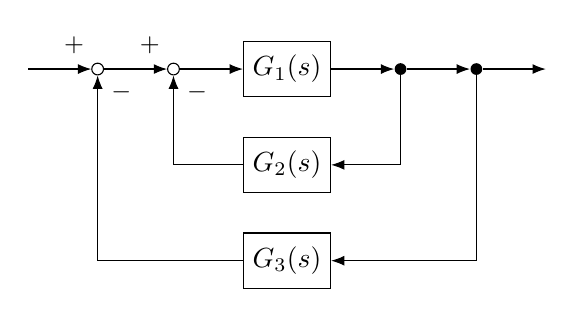
\begin{tikzpicture}[auto, node distance=0.8cm and 0.8cm, >=Latex]

      % --- 上段ノード ---
      \node[input] (input) {};
      \node[circle, draw, inner sep=1.5pt, right=of input] (sum1) {};           % 合流点①
      \node[circle, draw, inner sep=1.5pt, right=of sum1] (sum2) {}; % 合流点②
      \node[block, right=of sum2] (G1) {$G_1(s)$};              % G1
      \node[circle, fill=black, inner sep=1.5pt, right=of G1] (branch1) {}; % 分岐点①
      \node[circle, fill=black, inner sep=1.5pt, right=of branch1] (branch2) {}; % 分岐点②
      \node[output, right=of branch2] (output) {};
    
      % --- 下段ノード ---
      \node[block, below=0.5cm of G1] (G2) {$G_2(s)$};     % G2
      \node[block, below=0.5cm of G2] (G3) {$G_3(s)$};     % G3
    
      % --- 線描画 ---
      \draw[->] (input) -- (sum1);
      \draw[->] (sum1) -- (sum2);
      \draw[->] (sum2) -- (G1);
      \draw[->] (G1) -- (branch1);
      \draw[->] (branch1) -- (branch2);
      \draw[->] (branch2) -- (output);
    
      \draw[->] (branch1) |- (G2);        % 下向き:G2
      \draw[->] (G2) -| (sum2);          % 上に戻る:sum2
    
      \draw[->] (branch2) |- (G3);        % 下向き:G3
      \draw[->] (G3) -| (sum1);          % 上に戻る:sum1
    
      % --- 加算記号 ---
      \node at ($(sum1)+(-0.3,0.3)$) {\small $+$};
      \node at ($(sum1)+(0.3,-0.3)$) {\small $-$};
      \node at ($(sum2)+(-0.3,0.3)$) {\small $+$};
      \node at ($(sum2)+(0.3,-0.3)$) {\small $-$};
    
    \end{tikzpicture}
  \end{center}
\end{minipage}
\hfill
\begin{minipage}[t]{0.45\linewidth}
(2)
  \begin{center}
    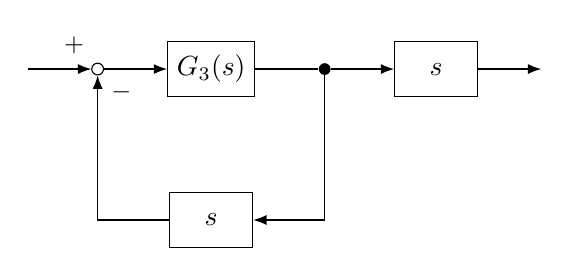
\begin{tikzpicture}[auto, node distance=0.8cm and 0.8cm, >=Latex]

      % --- 上段ノード ---
      \node[input] (input) {};
      \node[circle, draw, inner sep=1.5pt, right=of input] (sum) {};            % 合流点
      \node[block, right=of sum] (G3) {$G_3(s)$};                               % G_3(s)
      \node[circle, fill=black, inner sep=1.5pt, right=of G3] (branch) {};      % 分岐点
      \node[block, right=of branch] (S1) {$s$};                                 % 上の S
      \node[output, right=of S1] (output) {};
    
      % --- 下段ノード ---
      \node[block, below=1.2cm of G3] (S2) {$s$};                                % 下の S
    
      % --- 線描画 ---
      \draw[->] (input) -- (sum);
      \draw[->] (sum) -- (G3);
      \draw[-] (G3) -- (branch);
      \draw[->] (branch) -- (S1);
      \draw[->] (S1) -- (output);
    
      \draw[->] (branch) |- (S2);        % 分岐点から下のSへ
      \draw[->] (S2) -| (sum);           % 下のSから合流点へ
    
      % --- 加算記号 ---
      \node at ($(sum)+(-0.3,0.3)$) {\small $+$};
      \node at ($(sum)+(0.3,-0.3)$) {\small $-$};
    
    \end{tikzpicture}
  \end{center}
  
\end{minipage}\\

\begin{tcolorbox}[title={2. (1)
    \begin{center}
        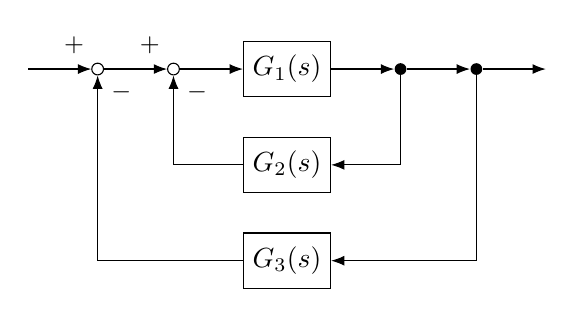
\begin{tikzpicture}[auto, node distance=0.8cm and 0.8cm, >=Latex]

        % --- 上段ノード ---
        \node[input] (input) {};
        \node[circle, draw, inner sep=1.5pt, right=of input] (sum1) {};           % 合流点①
        \node[circle, draw, inner sep=1.5pt, right=of sum1] (sum2) {}; % 合流点②
        \node[block, right=of sum2] (G1) {$G_1(s)$};              % G1
        \node[circle, fill=black, inner sep=1.5pt, right=of G1] (branch1) {}; % 分岐点①
        \node[circle, fill=black, inner sep=1.5pt, right=of branch1] (branch2) {}; % 分岐点②
        \node[output, right=of branch2] (output) {};
        
        % --- 下段ノード ---
        \node[block, below=0.5cm of G1] (G2) {$G_2(s)$};     % G2
        \node[block, below=0.5cm of G2] (G3) {$G_3(s)$};     % G3
        
        % --- 線描画 ---
        \draw[->] (input) -- (sum1);
        \draw[->] (sum1) -- (sum2);
        \draw[->] (sum2) -- (G1);
        \draw[->] (G1) -- (branch1);
        \draw[->] (branch1) -- (branch2);
        \draw[->] (branch2) -- (output);
        
        \draw[->] (branch1) |- (G2);        % 下向き:G2
        \draw[->] (G2) -| (sum2);          % 上に戻る:sum2
        
        \draw[->] (branch2) |- (G3);        % 下向き:G3
        \draw[->] (G3) -| (sum1);          % 上に戻る:sum1
        
        % --- 加算記号 ---
        \node at ($(sum1)+(-0.3,0.3)$) {\small $+$};
        \node at ($(sum1)+(0.3,-0.3)$) {\small $-$};
        \node at ($(sum2)+(-0.3,0.3)$) {\small $+$};
        \node at ($(sum2)+(0.3,-0.3)$) {\small $-$};
        
        \end{tikzpicture}
    \end{center} }]

\begin{center}
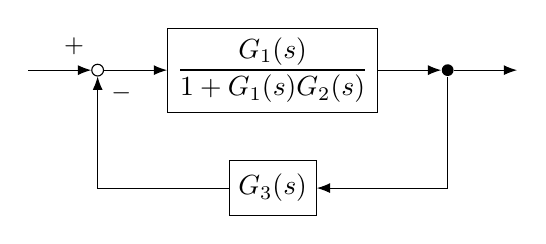
\begin{tikzpicture}[auto, node distance=0.8cm and 0.8cm, >=Latex]

  % --- 上段ノード ---
  \node[input] (input) {};
  \node[circle, draw, inner sep=1.5pt, right=of input] (sum1) {};              % 合流点①
  \node[block, right=of sum1] (G1G2) {$\dfrac{G_1(s)}{1 + G_1(s) G_2(s)}$};    % G1+G2合成済
  \node[circle, fill=black, inner sep=1.5pt, right=of G1G2] (branch2) {};      % 分岐点②
  \node[output, right=of branch2] (output) {};

  % --- 下段ノード ---
  \node[block, below=0.6cm of G1G2] (G3) {$G_3(s)$};

  % --- 線描画 ---
  \draw[->] (input) -- (sum1);
  \draw[->] (sum1) -- (G1G2);
  \draw[->] (G1G2) -- (branch2);
  \draw[->] (branch2) -- (output);

  \draw[->] (branch2) |- (G3);
  \draw[->] (G3) -| (sum1);

  % --- 加算記号 ---
  \node at ($(sum1)+(-0.3,0.3)$) {\small $+$};
  \node at ($(sum1)+(0.3,-0.3)$) {\small $-$};

\end{tikzpicture}


\vspace{2mm}
    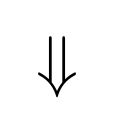
\begin{tikzpicture}
    \node {\Huge$\Downarrow$};
    \end{tikzpicture}
\vspace{2mm}


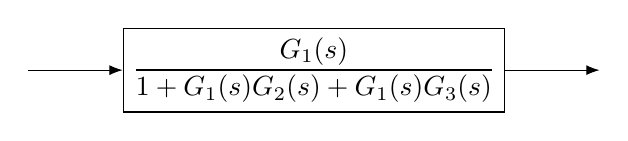
\begin{tikzpicture}[auto, node distance=1.5cm and 1.2cm, >=Latex]

  % --- ノード配置 ---
  \node[input] (input) {};
  \node[block, right=of input] (Gfinal) {$\dfrac{G_1(s)}{1 + G_1(s) G_2(s) + G_1(s) G_3(s)}$};
  \node[output, right=of Gfinal] (output) {};

  % --- 線描画 ---
  \draw[->] (input) -- (Gfinal);
  \draw[->] (Gfinal) -- (output);

\end{tikzpicture}
\end{center}

よってシステム全体の伝達関数は\\
\[
G_{all}(s)=\dfrac{G_1(s)}{1 + G_1(s) G_2(s) + G_1(s) G_3(s)}
\]


\end{tcolorbox}

\begin{tcolorbox}[title={2. (2)
    \begin{center}
    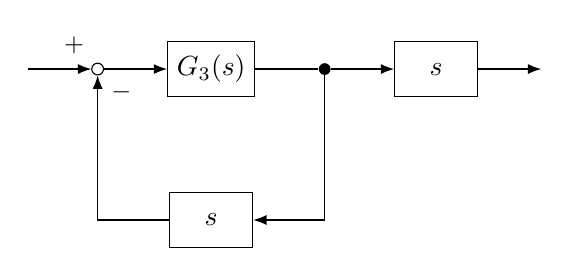
\begin{tikzpicture}[auto, node distance=0.8cm and 0.8cm, >=Latex]

        % --- 上段ノード ---
        \node[input] (input) {};
        \node[circle, draw, inner sep=1.5pt, right=of input] (sum) {};            % 合流点
        \node[block, right=of sum] (G3) {$G_3(s)$};                               % G_3(s)
        \node[circle, fill=black, inner sep=1.5pt, right=of G3] (branch) {};      % 分岐点
        \node[block, right=of branch] (S1) {$s$};                                 % 上の S
        \node[output, right=of S1] (output) {};

        % --- 下段ノード ---
        \node[block, below=1.2cm of G3] (S2) {$s$};                                % 下の S

        % --- 線描画 ---
        \draw[->] (input) -- (sum);
        \draw[->] (sum) -- (G3);
        \draw[-] (G3) -- (branch);
        \draw[->] (branch) -- (S1);
        \draw[->] (S1) -- (output);

        \draw[->] (branch) |- (S2);        % 分岐点から下のSへ
        \draw[->] (S2) -| (sum);           % 下のSから合流点へ

        % --- 加算記号 ---
        \node at ($(sum)+(-0.3,0.3)$) {\small $+$};
        \node at ($(sum)+(0.3,-0.3)$) {\small $-$};

    \end{tikzpicture}
    \end{center}}]

\begin{center}
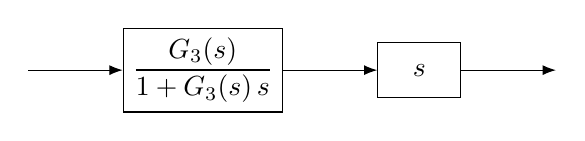
\begin{tikzpicture}[auto, node distance=0.8cm and 1.2cm, >=Latex]

  % --- ノード配置(不要ノード除去後) ---
  \node[input] (input) {};
  \node[block, right=of input] (G3fb) {$\dfrac{G_3(s)}{1 + G_3(s)\,s}$};
  \node[block, right=of G3fb] (S1) {$s$};
  \node[output, right=of S1] (output) {};

  % === 主系列 ===
  \draw[->] (input) -- (G3fb);
  \draw[->] (G3fb) -- (S1);
  \draw[->] (S1) -- (output);

\end{tikzpicture}

\vspace{2mm}
    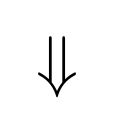
\begin{tikzpicture}
    \node {\Huge$\Downarrow$};
    \end{tikzpicture}
\vspace{2mm}


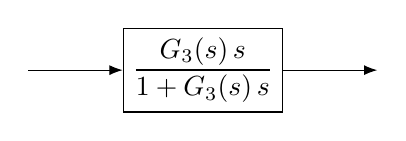
\begin{tikzpicture}[auto, node distance=1.5cm and 1.2cm, >=Latex]

  % --- ノード構成 ---
  \node[input] (input) {};
  \node[block, right=of input] (Gfinal) {$\dfrac{G_3(s)\,s}{1 + G_3(s)\,s}$};
  \node[output, right=of Gfinal] (output) {};

  % --- 線描画 ---
  \draw[->] (input) -- (Gfinal);
  \draw[->] (Gfinal) -- (output);

\end{tikzpicture}

\end{center}

よってシステム全体の伝達関数は\\
\[
G_{all}(s)=\dfrac{G_3(s)\,s}{1 + G_3(s)\,s}
\]


\end{tcolorbox}


% ---------------[3]--------------- 済
\begin{tcolorbox}[title={3. 問2.の(2)のシステムについて、\(G_3(s)=\dfrac{1}{s+3}\)のとき、単位ステップ入力を印加した際の応答を求めよ。
また、定常状態における値が存在すれば、その値を求めよ。}]

問2.の(2)より
\begin{align*}
G_{all}(s) &=  \dfrac{\frac{1}{s+3}\,s}{1 + \frac{1}{s+3}\,s} \\
            &= \dfrac{s}{2s+3}
\end{align*}
単位ステップ入力\(U(s)=\dfrac{1}{s}\)と\(Y(s)=G(S)U(S)\)より、
\begin{align*}
    &\qquad Y(s) =\frac{1}{2s+3} \\
    &\Leftrightarrow \mathcal{L}^{-1} \left[ Y(s) \right]
    =\mathcal{L}^{-1} \left[ \frac{1}{2s+3} \right]\\
    &\Leftrightarrow y(t) =  \frac{1}{2}e^{-\frac{3}{2}t}
\end{align*}
また定常値は
\[
\lim_{t \to \infty} y(t) = \lim_{t \to \infty} \frac{1}{2} e^{-\frac{3}{2}t} = 0
\]
\end{tcolorbox}

\newpage


% ---------------[4]---------------
\noindent
4. 以下の問に答えよ。なお、システムの入力を外力\(f(t)\)、出力を変位\(x(t)\)とし、
初期状態において系は静止しているとする。

\begin{center}
  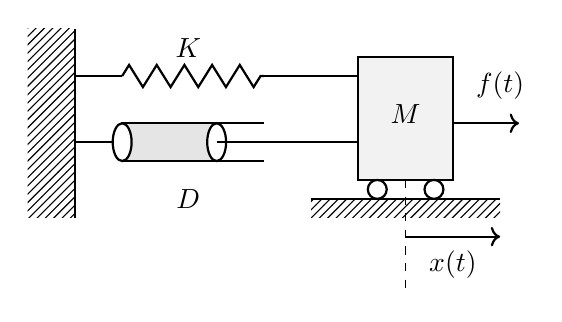
\begin{tikzpicture}[scale=1.2]
    % 固定壁
    \fill[pattern=north east lines] (-0.5,0) rectangle (0,2);
    \draw[thick] (0,0) -- (0,2);
  
    % バネ
    \draw[thick] (0,1.5) -- (0.5,1.5);
    \draw[thick, decorate, decoration={zigzag, segment length=10, amplitude=4}] (0.5,1.5) -- (2,1.5);
    \draw[thick] (2,1.5) -- (3.5,1.5);
    \node at (1.2,1.8) {$K$};
  
    % ダンパー(シリンダー形式)
    \draw[thick] (0,0.8) -- (0.5,0.8); % 棒
    \draw[thick, fill=gray!20] (0.5,0.6) rectangle (1.5,1.0); % 筒の側面
    \draw[thick] (1.5,1.0) -- (2,1.0); % 筒の上
    \draw[thick] (1.5,0.6) -- (2,0.6); % 筒の下
    \draw[thick, fill=white] (0.5,0.8) ellipse (0.1 and 0.2); % 左端面
    \draw[thick, fill=white] (1.5,0.8) ellipse (0.1 and 0.2); % 右端面
    \draw[thick] (1.5,0.8) -- (3,0.8); % ピストン棒
    \node at (1.2,0.2) {$D$};
  
    % 質量M
    \draw[thick, fill=gray!10] (3,0.4) rectangle (4,1.7);
    \node at (3.5,1.1) {$M$};
    % ローラー追加
      \draw[thick] (3.2,0.3) circle (0.1);
      \draw[thick] (3.8,0.3) circle (0.1);

  
    % 床
    \draw[thick] (2.5,0.2) -- (4.5,0.2);
    \fill[pattern=north east lines] (2.5,0) rectangle (4.5,0.2);
  
    % 座標
    \draw[->, thick] (3.5,-0.2) -- (4.5,-0.2);
    \node at (4,-0.5) {$x(t)$};
    \draw[dashed] (3.5,0.4) -- (3.5,-0.8);
  
    % 外力
    \draw[->, thick] (4,1) -- (4.7,1);
    \node at (4.5,1.4) {$f(t)$};
  \end{tikzpicture}
\end{center}

\indent
(1)上図によって示されるシステムの運動方程式ならびに伝達関数を求めよ。\\

\indent
(2)各パラメータを\(M=1,D=5,K=6\)として、インパルス応答を求めよ。\\

\indent
(3)問(2)のパラメータを用いて、単位ステップ応答\(x(t)\)を求めよ。\\

\indent
(4)単位ステップ応答の概形を描け。
なおグラフの横軸を時間\(t\),縦軸を変位\(x(t)\)とする。\\

\indent
(5)\(M=1,D=0,K=0,\)入力を\(f(t)=\sin \omega t\)として、応答\(x(t)\)を求めよ。\\

\indent
(6)\(M=1,D=0,K=2\)として、ステップ入力を与えたときの応答\(x(t)\)を求めよ。\\

\indent
(7)\(M=1,D=2,K=1,\)入力を\(f(t)=\sin \omega t\)として、応答\(x(t)\)を求めよ。\\

\indent
(8)\(M=1,D=4,K=5\)として、ステップ入力を与えたときの応答\(x(t)\)を求めよ。\\
% ---------------[4(1)]--------------- 済
\begin{tcolorbox}[title={4. (1) 上図によって示されるシステムの運動方程式ならびに伝達関数を求めよ。}]
    \(x(t)\)に関する運動方程式は
    \begin{align*}
        &\qquad M\ddot{x} =f(t) -Kx - D \dot{x} \\
    \end{align*}
    また伝達関数は
    \begin{align*}
        &\qquad M\ddot{x} + Kx + D \dot{x} =f(t) \\
        &\therefore \quad \mathcal{L} \left[ M\ddot{x} + D \dot{x} + Kx\right] 
        =\mathcal{L} \left[ f(t) \right] \\
        &\therefore \quad (M s^2 + D s + K)\,X(s) = F(s) \quad [\because \dot{x}(0)=x(0)=0 ]\\
        &\therefore \quad G(s) \;=\;\frac{X(s)}{F(s)}
        \;=\;\frac{1}{M s^2 + D s + K}
    \end{align*}
    
\end{tcolorbox}

% ---------------[4(2)]--------------- 済
\begin{tcolorbox}[title={4. (2) 各パラメータを\(M=1,D=5,K=6\)として、インパルス応答を求めよ。}]
     パラメータを代入し、インパルス入力のラプラス変換は\(F(s)=1\)なので
     \vspace{-2mm}
     \begin{align*}
        &\qquad G(s) = \frac{1}{s^2 + 5s + 6} \\
        &\therefore \quad X(s) = G(s) F(s) = \frac{1}{s^2 + 5s + 6}\\
        &\therefore \quad X(s) = \frac{1}{(s+2)(s+3)}\\
        &\therefore \quad X(s) = \frac{1}{s+2} - \frac{1}{s+3}\\
        &\therefore \quad \mathcal{L} \left[ X(s)\right] 
        =\mathcal{L} \left[ \frac{1}{s+2}\right] - \left[\frac{1}{s+3}  \right] \\
        &\therefore \quad x(t) = e^{-2t} - e^{-3t}
    \end{align*}
\end{tcolorbox}

% ---------------[4(3)]--------------- 済
\begin{tcolorbox}[title={4. (3) 問(2)のパラメータを用いて、単位ステップ応答\(x(t)\)を求めよ。}]
    パラメータを代入し、ステップ入力のラプラス変換は\(F(s)=\dfrac{1}{s}\)なので
     \vspace{-2mm}
     \begin{align*}
        &\qquad G(s) = \frac{1}{s^2 + 5s + 6} \\
        &\therefore \quad X(s) = G(s) F(s) = \frac{1}{s(s^2 + 5s + 6)}\\
        &\therefore \quad X(s) = \frac{1}{s(s+2)(s+3)}\\
        &\therefore \quad X(s) = \frac{(\frac{1}{6})}{s} 
        + \frac{(-\frac{1}{2})}{s+2} + \frac{(\frac{1}{3})}{s+3}\\
        &\therefore \quad \mathcal{L} \left[ X(s)\right] 
        =\mathcal{L} \left[\frac{(\frac{1}{6})}{s}\right] 
        + \left[\frac{(-\frac{1}{2})}{s+2} \right] + \left[\frac{(\frac{1}{3})}{s+3} \right] \\
        &\therefore \quad x(t) = \frac{1}{6} - \frac{1}{2} e^{-2t} + \frac{1}{3} e^{-3t}
    \end{align*}
\end{tcolorbox}

% ---------------[4(4)]--------------- 済
\begin{tcolorbox}[title={4. (4) 単位ステップ応答の概形を描け。
なおグラフの横軸を時間\(t\),縦軸を変位\(x(t)\)とする。}]
    \begin{center}
    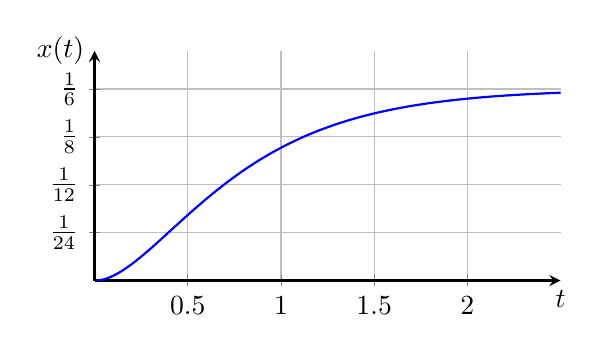
\begin{tikzpicture}
        \begin{axis}[
    axis lines = middle,
    xlabel = {$t$},
    ylabel = {$x(t)$},
    xmin=0, xmax=2.5,
    ymin=0, ymax=0.2,
    samples=300,
    domain=0:2.5,
    thick,
    width=7.5cm,
    height=4.5cm,
    grid=both,
    xtick={0,0.5,1,1.5,2},
    ytick={0,0.0417,0.0833,0.125,0.1667},
    yticklabels={$0$, $\frac{1}{24}$, $\frac{1}{12}$, $\frac{1}{8}$, $\frac{1}{6}$},
    every axis x label/.style={at={(current axis.right of origin)}, anchor=north},
    every axis y label/.style={at={(current axis.above origin)}, anchor=east},
]

        \addplot[blue, thick, domain=0:2.5] {(1/6) - (1/2)*exp(-2*x) + (1/3)*exp(-3*x)};
        \end{axis}
    \end{tikzpicture}
    \end{center}
\end{tcolorbox}

% ---------------[4(5)]--------------- 済
\begin{tcolorbox}[title={4. (5) \(M=1,D=0,K=0,\)入力を\(f(t)=\sin \omega t\)として、応答\(x(t)\)を求めよ。}]
    パラメータを代入し、\(F(s) = \dfrac{\omega}{s^2 + \omega^2}\)なので
    \vspace{-2mm}
    \begin{align*}
        &\qquad G(s) = \frac{1}{s^2} \\
        &\therefore \quad X(s) = G(s)F(s) 
        = \frac{\omega}{s^2(s^2 + \omega^2)} \\
        &\therefore \quad X(s) = \frac{(\frac{1}{\omega})}{s^2} 
        + \frac{-(\frac{1}{\omega})}{s^2 + \omega^2} \\
        &\therefore \quad \mathcal{L}^{-1}[X(s)] = \mathcal{L}^{-1}\left[\frac{(\frac{1}{\omega})}{s^2}\right]
        + \mathcal{L}^{-1}\left[\frac{-(\frac{1}{\omega})}{s^2 + \omega^2}\right] \\
        &\therefore \quad x(t) = \frac{1}{\omega} \left(t - \frac{1}{\omega} \sin \omega t \right)
    \end{align*}
\end{tcolorbox}

% ---------------[4(6)]--------------- 済
\begin{tcolorbox}[title={4. (6) \(M=1,D=0,K=2\)としてステップ入力を与えたときの応答\(x(t)\)を求めよ。}]
    パラメータを代入し、ステップ入力のラプラス変換は\(F(s)=\dfrac{1}{s}\)なので
    \vspace{-2mm}
    \begin{align*}
        &\qquad G(s) = \frac{1}{s^2 + 2} \\
        &\therefore \quad X(s) = G(s) F(s) = \frac{1}{s(s^2 + 2)} \\
        &\therefore \quad X(s) = \frac{(\frac{1}{2})}{s} + \frac{-(\frac{1}{2}s)}{s^2 + 2} \\
        &\therefore \quad \mathcal{L}^{-1} \left[ X(s)\right] 
        = \mathcal{L}^{-1} \left[\frac{(\frac{1}{2})}{s}\right] 
        + \mathcal{L}^{-1} \left[ \frac{-(\frac{1}{2}s)}{s^2 + 2} \right] \\
        &\therefore \quad x(t) = \frac{1}{2}\left\{1 - \cos(\sqrt{2}t) \right\} = \sin ^2 \left( \frac{t}{\sqrt{2}} \right)
    \end{align*}
\end{tcolorbox}

% ---------------[4(7)]--------------- 済
\begin{tcolorbox}[title={4. (7) \(M=1,D=2,K=1,\)入力を\(f(t)=\sin \omega t\)として、応答\(x(t)\)を求めよ。}]
    パラメータを代入し、\(F(s) = \dfrac{\omega}{s^2 + \omega^2}\)なので
    \vspace{-2mm}
    \begin{align*}
        &\qquad G(s) = \frac{1}{s^2 + 2s + 1} \\
        &\therefore \quad X(s) = G(s) F(s) = \frac{\omega}{(s+1)^2(s^2 + \omega^2)} \\
        &\therefore \quad X(s) 
        = \dfrac{\left(\dfrac{\omega}{\omega^2 + 1}\right)}{(s+1)^2}
        + \dfrac{\left(\dfrac{2}{(\omega^2 + 1)^2}\right)}{s+1}
        + \dfrac{\left(\dfrac{-2 \omega s - \omega^3 + \omega}{(1+\omega^2)^2}\right)}{s^2+\omega^2} \\
        &\therefore \quad \mathcal{L}^{-1} \left[ X(s)\right]\\ 
        & \quad = \frac{1}{(\omega^2 + 1)^2} \left\{ \mathcal{L}^{-1} \left[\frac{\omega(\omega^2 + 1)}{(s+1)^2}\right]
        + \mathcal{L}^{-1} \left[\frac{2}{s+1}\right]
        + \mathcal{L}^{-1} \left[\frac{-2 \omega s-\omega ^3+\omega}{s^2+\omega^2}\right] 
        \right\}\\
        &\therefore \quad x(t) =\frac{1}{(\omega^2 + 1)^2}
        \left\{\omega (\omega^2+1)  t e^{-t}+ 2 e^{-t}
        - 2\omega \cos(\omega t) + (1 - \omega^2)  \sin(\omega t) 
        \right\}
    \end{align*}
\end{tcolorbox}

% ---------------[4(8)]--------------- 済
\begin{tcolorbox}[title={4. (8) \(M=1,D=4,K=5\)としてステップ入力を与えたときの応答\(x(t)\)を求めよ。}]
    パラメータを代入し、\(F(s) = \dfrac{1}{s}\)なので
    \vspace{-2mm}
  \begin{align*}
    &\qquad G(s) = \frac{1}{s^2 + 4s + 5} \\
    &\therefore\quad X(s) = \frac{1}{s(s^2 + 4s + 5)} \\
    &\therefore\quad X(s) = \frac{\left(\frac{1}{5}\right)}{s} 
    + \frac{\left(-\frac{s}{5}-\frac{4}{5}\right)}{s^2 + 4s + 5} \\
    &\therefore\quad X(s) = \frac{1}{5s} - \frac{1}{5} \cdot \frac{(s + 2) + 2}{(s + 2)^2 + 1} \\
    &\therefore \quad \mathcal{L}^{-1} \left[ X(s)\right] \\
    &\quad = \mathcal{L}^{-1} \left[\frac{1}{5s}\right] 
    - \frac{1}{5} \mathcal{L}^{-1} \left[\frac{1}{5} \cdot \frac{s + 2}{(s + 2)^2 + 1}\right]
    - \frac{1}{5} \mathcal{L}^{-1} \left[\frac{1}{5} \cdot \frac{2}{(s + 2)^2 + 1} \right] \\
    &\therefore\quad x(t) = \frac{1}{5} - \frac{1}{5} e^{-2t} \cos t - \frac{2}{5} e^{-2t} \sin t
\end{align*}
\end{tcolorbox}

% ---------------[5]---------------
\begin{tcolorbox}[title={5.下図に示すフィードバックシステムにおいて、\(G_1(s)=\dfrac{1}{s+2},G_2(s)=s,G_3(s)=K_1\)
となるとき、ステップ応答における定常値が1になるよう、\(K_1\)を定めよ。\\
\begin{center}
  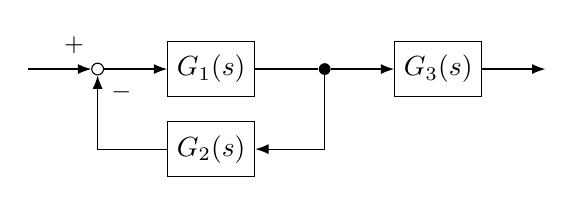
\begin{tikzpicture}[auto, node distance=0.8cm and 0.8cm, >=Latex]

    % --- 上段ノード ---
    \node[input] (input) {};
    \node[circle, draw, inner sep=1.5pt, right=of input] (sum) {};            % 合流点
    \node[block, right=of sum] (G3) {$G_1(s)$};                               % G_3(s)
    \node[circle, fill=black, inner sep=1.5pt, right=of G3] (branch) {};      % 分岐点
    \node[block, right=of branch] (S1) {$G_3(s)$};                                 % 上の S
    \node[output, right=of S1] (output) {};
  
    % --- 下段ノード ---
    \node[block, below=0.3cm of G3] (S2) {$G_2(s)$};                                % 下の S
  
    % --- 線描画 ---
    \draw[->] (input) -- (sum);
    \draw[->] (sum) -- (G3);
    \draw[-] (G3) -- (branch);
    \draw[->] (branch) -- (S1);
    \draw[->] (S1) -- (output);
  
    \draw[->] (branch) |- (S2);        % 分岐点から下のSへ
    \draw[->] (S2) -| (sum);           % 下のSから合流点へ
  
    % --- 加算記号 ---
    \node at ($(sum)+(-0.3,0.3)$) {\small $+$};
    \node at ($(sum)+(0.3,-0.3)$) {\small $-$};
  
  \end{tikzpicture}
\end{center}}]
\begin{center}
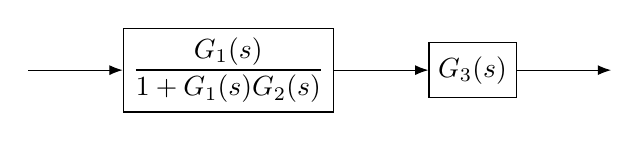
\begin{tikzpicture}[auto, node distance=0.8cm and 1.2cm, >=Latex]

  % --- ノード構成 ---
  \node[input] (input) {};
  \node[block, right=of input] (G1G2) {$\dfrac{G_1(s)}{1 + G_1(s) G_2(s)}$};
  \node[block, right=of G1G2] (G3) {$G_3(s)$};
  \node[output, right=of G3] (output) {};

  % --- 線描画 ---
  \draw[->] (input) -- (G1G2);
  \draw[->] (G1G2) -- (G3);
  \draw[->] (G3) -- (output);

\end{tikzpicture}

\vspace{2mm}
    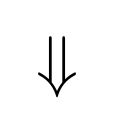
\begin{tikzpicture}
    \node {\Huge$\Downarrow$};
    \end{tikzpicture}
\vspace{2mm}

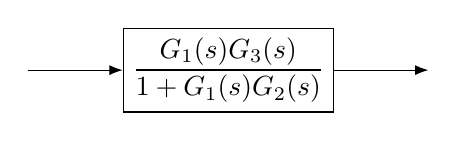
\begin{tikzpicture}[auto, node distance=1.5cm and 1.2cm, >=Latex]

  % --- ノード構成 ---
  \node[input] (input) {};
  \node[block, right=of input] (Gfinal) {$\dfrac{G_1(s) G_3(s)}{1 + G_1(s) G_2(s)}$};
  \node[output, right=of Gfinal] (output) {};

  % --- 線描画 ---
  \draw[->] (input) -- (Gfinal);
  \draw[->] (Gfinal) -- (output);

\end{tikzpicture}
\end{center}
\vspace{-4mm}
よってシステム全体の伝達関数は
\vspace{-4mm}
\begin{align*}
  G_{all}(s) &=\dfrac{G_1(s) G_3(s)}{1 + G_1(s) G_2(s)} \\
            & =\dfrac{\frac{1}{s+2} K_1}{1 +\frac{1}{s+2} \cdot s} \\
            & =\dfrac{K_1}{2(s+1)}
\end{align*}
単位ステップ入力\(U(s)=\frac{1}{s}\)とすると、単位ステップ応答\(X(s)\)は
\vspace{-3mm}
\begin{align*}
    &\qquad X(s) =G_{all}(s) U(s)=\dfrac{K_1}{2s(s+1)} \\
    &\Leftrightarrow X(s) = \frac{K_1}{2}\left(\frac{1}{s} - \frac{1}{s+1} \right) \\
    &\Leftrightarrow \mathcal{L}^{-1} \left[ X(s)  \right]
    =\mathcal{L}^{-1} \left[ \frac{K_1}{2}\left(\frac{1}{s} - \frac{1}{s+1} \right) \right]\\
    &\Leftrightarrow x(t) =  \frac{K_1}{2} \left(1-e^{-t} \right)
\end{align*}
また定常値は
\[
\lim_{t \to \infty} x(t) = \lim_{t \to \infty} \frac{K_1}{2} \left(1-e^{-t} \right) = \frac{K_1}{2}
\]
よって定常値が1になるような\(K_1\)は
\vspace{-3mm}
\[
K_1=2
\]
  \begin{tcolorbox}[title={}]
  ※最終値定理より以下のように解く方が速い
  \[
  \lim_{t \to \infty} x(t) = \lim_{s \to 0} sX(s) = \frac{K_1}{2} \therefore K_1=2
  \]
  \end{tcolorbox}
\end{tcolorbox}

\newpage

% ---------------[6]---------------
\noindent
6.次の微分方程式について、初期値をすべて0として、\(x(t)\)を求めよ。\\

(1)\quad \( \ddot{x}(t)+ 2\dot{x}+ 2x(t)= \sin 2t \)\\

(2)\quad \( \dot{x}(t)+ x(t)= 1(t)- 1(t-2) \)\\

\vspace{2mm}

\begin{tcolorbox}[title={6.(1) \( \ddot{x}(t)+ 2\dot{x}+ 2x(t)= \sin 2t \)
    }]
    \quad 両辺にラプラス変換を施すと,
    \vspace{-3mm}
    \begin{align*}
        &\qquad \mathcal{L}\left[ \ddot{x}(t)+ 2\dot{x}+ 2x(t) \right] 
        = \mathcal{L} \left[ \sin 2t \right] \\
        &\Leftrightarrow \left\{ s^2 X(s) - sx(0) - \dot{x}(0) \right\}
        + 2 \left\{ sX(s) - x(0) \right\}
        + 2 X(s) = \frac{2}{s^2+2^2}  \\
        &\Leftrightarrow s^2 X(s) + 2sX(s) + 2 X(s) = \frac{2}{s^2+2^2}  \\
        &\Leftrightarrow X(s) = \frac{2}{(s^2+2^2)(s^2+2s+2)}  \\
        &\Leftrightarrow X(s) = \frac{-\frac{1}{5}s-\frac{1}{5}}{(s^2+2^2)} + \frac{\frac{1}{5}s+\frac{3}{5}}{(s^2+2s+2)}\\
        &\Leftrightarrow X(s) = -\frac{1}{5} \frac{s+\frac{1}{2} \cdot 2}{(s^2+2^2)} + \frac{1}{5} \frac{(s+1)+2}{((s+1)^2+1)}
    \end{align*}
        
    \quad 両辺にラプラス逆変換を施すと,
    \vspace{-3mm}
    \begin{align*}
    &\qquad \mathcal{L}^{-1} \left[ X(s) \right] 
    = \mathcal{L}^{-1} \left[ -\frac{1}{5} \frac{s+\frac{1}{2} \cdot 2}{(s^2+2^2)}   \right] 
    + \mathcal{L}^{-1} \left[ \frac{1}{5} \frac{(s+1)+2}{((s+1)^2+1)}  \right] \\
    &\Leftrightarrow x(t) = -\frac{1}{5}\left\{ \cos 2t + \frac{1}{2} \sin 2t \right\}
    + \frac{1}{5}e^{-t}\left\{\cos t + \sin 2t\right\}
    \end{align*}
\end{tcolorbox}

\begin{tcolorbox}[title={6.(2) \( \dot{x}(t)+ x(t)= 1(t)- 1(t-2) \)
    }]
    \quad 両辺にラプラス変換を施すと,
    \vspace{-3mm}
    \begin{align*}
        &\qquad \mathcal{L}\left[ \dot{x}(t)+ x(t) \right] 
        = \mathcal{L} \left[ 1(t)- 1(t-2) \right] \\
        &\Leftrightarrow \left\{ sX(s) - x(0) \right\} + X(s) 
        = \frac{1}{s} - \frac{e^{-2s}}{s} \quad 
        \left[\because \int_{-\infty}^{\infty} f(t)\delta(t-a) dt = f(a)\right]\\
        &\Leftrightarrow X(s) = \frac{1}{s(s+1)} - \frac{e^{-2s}}{s(s+1)}  \\
        &\Leftrightarrow X(s) = \frac{1}{s} - \frac{1}{s+1} 
        - \left\{ \frac{e^{-2s}}{s} - \frac{e^{-2s}}{s+1} \right\} 
    \end{align*}
        
    \quad 両辺にラプラス逆変換を施すと,
    \vspace{-3mm}
    \begin{align*}
    &\qquad \mathcal{L}^{-1} \left[ X(s) \right] 
    = \mathcal{L}^{-1} \left[ \frac{1}{s} - \frac{1}{s+1}   \right] 
    - \mathcal{L}^{-1} \left[ \left\{ \frac{e^{-2s}}{s} - \frac{e^{-2s}}{s+1} \right\}  \right] \\
    &\Leftrightarrow x(t) = 1-e^{-t} - \left\{1-e^{-(t-2)}\right\} 1(t-2)
    \end{align*}
\end{tcolorbox}


\newpage

% ---------------[7]---------------
\noindent
7.下図に示すシステムについて、入力を変位\(x_i(t),\)出力を変位\(x_o(t)\)としたとき、
次の問に答えよ。なお、\(m\)は質量[kg]、\(d\)は粘性係数[Ns/m]、kはバネ定数[N/m]とし、
初期状態において系は静止しているとする。
  \begin{center}
    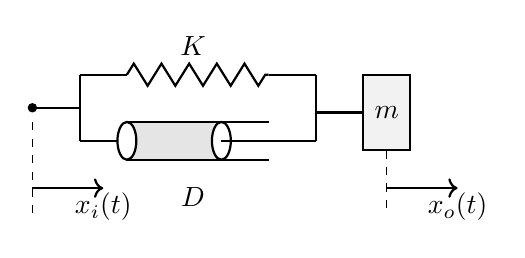
\begin{tikzpicture}[scale=1.2]
      % バネ
      \draw[thick] (0,1.5) -- (0.5,1.5);
      \draw[thick, decorate, decoration={zigzag, segment length=10, amplitude=4}] (0.5,1.5) -- (2,1.5);
      \draw[thick] (2,1.5) -- (2.5,1.5);
      \node at (1.2,1.8) {$K$};
    
      % ダンパー(シリンダー形式)
      \draw[thick] (0,0.8) -- (0.5,0.8); % 棒
      \draw[thick, fill=gray!20] (0.5,0.6) rectangle (1.5,1.0); % 筒の側面
      \draw[thick] (1.5,1.0) -- (2,1.0); % 筒の上
      \draw[thick] (1.5,0.6) -- (2,0.6); % 筒の下
      \draw[thick, fill=white] (0.5,0.8) ellipse (0.1 and 0.2); % 左端面
      \draw[thick, fill=white] (1.5,0.8) ellipse (0.1 and 0.2); % 右端面
      \draw[thick] (1.5,0.8) -- (2.5,0.8); % ピストン棒
      \node at (1.2,0.2) {$D$};

      %接続部分
      \draw[thick] (2.5,1.5) -- (2.5,0.8);
      \draw[thick] (2.5,1.1) -- (3.0,1.1);

      % 質量m
      \draw[thick, fill=gray!10] (3,0.7) rectangle (3.5,1.5);
      \node at (3.25,1.1) {$m$};

      % 座標
      \draw[->, thick] (3.25,0.3) -- (4,0.3);
      \node at (4,0.1) {$x_o(t)$};
      \draw[dashed] (3.25,0.7) -- (3.25,0);

      \draw[->, thick] (-0.5,0.3) -- (0.25,0.3);
      \node at (0.25,0.1) {$x_i(t)$};
      \draw[dashed] (-0.5,1) -- (-0.5,0);

      \draw[thick] (0,0.8) -- (0,1.5);
      \draw[thick] (0,1.15) -- (-0.5,1.15);

      \fill (-0.5,1.15) circle (0.05);
    \end{tikzpicture}
  \end{center}

\indent
(1)システムの運動方程式を求めよ。\\

\indent
(2)システムの伝達関数を求めよ。\\

\indent
(3)インパルス入力を印加した際の定常値を求めよ。\\

\indent
(4)ステップ入力を印加した際の定常値を求めよ。\\

\indent
(5)\quad \( m=1,d=3,k=2\)とし、インパルス応答、ステップ応答をそれぞれ求めよ。\\

\indent
(6)\quad \( m=1,d=0,k=1\)とし、ステップ応答を求めよ。\\

\indent
(7)\quad \( m=1,d=2,k=3\)とし、ステップ応答を求めよ。\\

\indent
(8)\quad \( m=1,d=2,k=1\)とし、入力\(x_1(t)=\sin (t)\) を印加したときの応答を求めよ。\\

\indent
(9)\quad \( m=1,d=1,k=0\)とし、入力\(x_1(t)=\cos (t)\) を印加したときの応答を求めよ。\\

% ---------------[7(1)]--------------- 済
\begin{tcolorbox}[title={7.(1)システムの運動方程式を求めよ。
    }]
    \(x(t)\)に関する運動方程式は
    \begin{align*}
        &\qquad m\ddot{x}_0 = -k(x_o - x_i)  - d (\dot{x}_o - \dot{x}_i)
    \end{align*}
\end{tcolorbox}
% ---------------[7(2)]--------------- 済
\begin{tcolorbox}[title={7.(2)システムの伝達関数を求めよ。
    }]
    伝達関数は
    \begin{align*}
        &\qquad m\ddot{x}_0 = -k(x_o - x_i)  - D (\dot{x}_o - \dot{x}_i) \\
        &\qquad m\ddot{x}_o + D \dot{x}_o + kx_o =  D \dot{x}_i + kx_i \\
        &\therefore \quad \mathcal{L} \left[ M\ddot{x}_o + D \dot{x}_o + kx_o \right] 
        =\mathcal{L} \left[ D \dot{x}_i + kx_i \right] \\
        &\therefore \quad (m s^2 + D s + k)\,X_o(s) =(D s + k)X_i(s) \quad [\because \text{初期値はすべてゼロ}]\\
        &\therefore \quad G(s) \;=\;\frac{X_o(s)}{X_i(s)}
        \;=\;\frac{D s + k}{m s^2 + D s + k}
    \end{align*}
\end{tcolorbox}
% ---------------[7(3)]--------------- 済
\begin{tcolorbox}[title={7.(3)インパルス入力を印加した際の定常値を求めよ。
    }]
    インパルス入力のラプラス変換は\(X_i(s)=1\)なので
    \vspace{-2mm}
    \begin{align*}
        &\qquad G(s) = \frac{d s + k}{m s^2 + d s + k} \\
        &\therefore \quad X_o(s) = G(s) X_i(s) = \frac{d s + k}{m s^2 + d s + k}
    \end{align*}
    最終値定理より
    \begin{align*}
    \lim_{t \to \infty} x_o(t) &= \lim_{s \to 0} sX_o(s) \\
        &= \lim_{s \to 0} \frac{d s^2 + ks}{m s^2 + d s + k} \\
        &= 0
    \end{align*}
    \begin{tcolorbox}[title={}]
      ※\(x_o\)を強引に求めてから定常値を求める方法 (非推奨)
        \vspace{-2mm}
        \begin{align*}
          &\qquad  \quad X_o(s) = \frac{d s + k}{m s^2 + d s + k}\\
          &\therefore \quad X_o(s) = \frac{\frac{d}{m} s + \frac{k}{m}}{s^2 + \frac{d}{m} s + \frac{k}{m}} \quad \left[\because m \neq 0\right]\\
          &\therefore \quad X_o(s) = \frac{2A s + B^2}{s^2 + 2A s + B^2} \quad \left[A=\frac{d}{2m},B=\sqrt{\frac{k}{m}}\right]\\
          &\therefore \quad X_o(s) = \frac{2A s + B^2}{(s+A)^2+B^2-A^2}\\
          &\therefore \quad X_o(s) = \frac{2A (s+A)}{(s+A)^2+B^2-A^2}
          + \frac{B^2-2A^2}{(s+A)^2+B^2-A^2} 
        \end{align*}
      \quad 両辺にラプラス逆変換を施すと,
        \vspace{-3mm}
        \begin{align*}
        &\qquad \mathcal{L}^{-1} \left[ X_o(s) \right] 
        = \mathcal{L}^{-1} \left[ \frac{2A (s+A)}{(s+A)^2+B^2-A^2}  \right]
        + \mathcal{L}^{-1} \left[ \frac{B^2-2A^2}{(s+A)^2+B^2-A^2}  \right]\\
        &\Leftrightarrow x_o(t) = 2A e^{-At} \cos (\sqrt{B^2-A^2}t) + \frac{B^2-2A^2}{\sqrt{B^2-A^2}} e^{-At} \sin (\sqrt{B^2-A^2}t)
        \end{align*}
        以上より定常値は
        \vspace{-3mm}
        \begin{align*}
        \lim_{t \to \infty} x_o(t) 
            &= \lim_{t \to \infty} \left\{2A e^{-At} \cos (\sqrt{B^2-A^2}t) \right.\\
            &\qquad \qquad + \left.\frac{B^2-2A^2}{\sqrt{B^2-A^2}} e^{-At} \sin (\sqrt{B^2-A^2}t) \right\}\\
            &= 0
        \end{align*}
    \end{tcolorbox}
\end{tcolorbox}
% ---------------[7(4)]--------------- 済
\begin{tcolorbox}[title={7.(4)ステップ入力を印加した際の定常値を求めよ。
    }]
        ステップ入力のラプラス変換は\(X_i(s)=\frac{1}{s}\)なので
    \vspace{-2mm}
    \begin{align*}
        &\qquad G(s) = \frac{d s + k}{m s^2 + d s + k} \\
        &\therefore \quad X_o(s) = G(s) X_i(s) = \frac{d s + K}{s(m s^2 + d s + k)}\\
    \end{align*}
    最終値定理より
    \begin{align*}
    \lim_{t \to \infty} x_o(t) &= \lim_{s \to 0} sX_o(s) \\
        &= \lim_{s \to 0} \frac{d s + k}{m s^2 + d s + k} \\
        &= 1
    \end{align*}
※\(x_0(t)\) を強引に求める方法は、7.(3)の面倒さにさらに部分分数分解の面倒さも加わるので、再現性はない。
\end{tcolorbox}
% ---------------[7(5)]--------------- 済
\begin{tcolorbox}[title={7.(5)\quad \( m=1,d=3,k=2\)とし、インパルス応答、ステップ応答をそれぞれ求めよ。
    }]
    (\uppercase\expandafter{\romannumeral 1})インパルス応答 \\
    パラメータを代入し、インパルス入力のラプラス変換は\(F(s)=1\)なので
    \vspace{-2mm}
    \begin{align*}
        &\qquad G(s) = \frac{3 s + 2}{s^2 + 3 s + 2} \\
        &\therefore \quad X(s) = G(s) F(s) = \frac{3 s + 2}{(s+1)(s+2)} \\
        &\therefore \quad X(s) = \frac{-1}{s+1} + \frac{4}{s+2} \\
        &\therefore \quad \mathcal{L}^{-1} \left[ X(s)\right] 
        = \mathcal{L}^{-1} \left[\frac{-1}{s+1}\right] 
        + \mathcal{L}^{-1} \left[\frac{4}{s+2} \right] \\
        &\therefore \quad x(t) = -e^{-t} + 4 e^{-2t}
    \end{align*}

    (\uppercase\expandafter{\romannumeral 2})ステップ応答 \\
    パラメータを代入し、ステップ入力のラプラス変換は\(F(s)=\dfrac{1}{s}\)なので
    \vspace{-2mm}
    \begin{align*}
        &\qquad G(s) = \frac{3 s + 2}{s^2 + 3 s + 2} \\
        &\therefore \quad X(s) = G(s) F(s) = \frac{3 s + 2}{s(s+1)(s+2)} \\
        &\therefore \quad X(s) = \frac{1}{s}+\frac{1}{s+1} + \frac{-2}{s+2} \\
        &\therefore \quad \mathcal{L}^{-1} \left[ X(s)\right] 
        = \mathcal{L}^{-1} \left[\frac{1}{s}\right] 
        + \mathcal{L}^{-1} \left[\frac{1}{s+1} \right]
        + \mathcal{L}^{-1} \left[\frac{-2}{s+2} \right] \\
        &\therefore \quad x(t) = 1 + e^{-t} -2 e^{-2t}
    \end{align*}
\end{tcolorbox}
% ---------------[7(6)]--------------- 済
\begin{tcolorbox}[title={7.(6)\quad \( m=1,d=0,k=1\)とし、ステップ応答を求めよ。
    }]
    パラメータを代入し、ステップ入力のラプラス変換は\(F(s)=\dfrac{1}{s}\)なので
    \vspace{-4mm}
    \begin{align*}
        &\qquad G(s) = \frac{1}{s^2 + 1} \\
        &\therefore \quad X(s) = G(s) F(s) = \frac{1}{s(s^2+1)} \\
        &\therefore \quad X(s) = \frac{1}{s}+\frac{-s}{s^2+1} \\
        &\therefore \quad \mathcal{L}^{-1} \left[ X(s)\right] 
        = \mathcal{L}^{-1} \left[\frac{1}{s}\right] 
        + \mathcal{L}^{-1} \left[\frac{-s}{s^2+1} \right] \\
        &\therefore \quad x(t) = 1 - \cos t
    \end{align*}
\end{tcolorbox}
% ---------------[7(7)]--------------- 済
\begin{tcolorbox}[title={7.(7)\quad \( m=1,d=2,k=3\)とし、ステップ応答を求めよ。
    }]
    パラメータを代入し、ステップ入力のラプラス変換は\(F(s)=\dfrac{1}{s}\)なので
    \vspace{-4mm}
    \begin{align*}
        &\qquad G(s) = \frac{2s+3}{s^2 + 2s+ 3} \\
        &\therefore \quad X(s) = G(s) F(s) = \frac{2s+3}{s\left\{(s+1)^2+2\right\}} \\
        &\therefore \quad X(s) = \frac{1}{s}+\frac{-s}{(s+1)^2+2} \\
        &\therefore \quad \mathcal{L}^{-1} \left[ X(s)\right] 
        = \mathcal{L}^{-1} \left[\frac{1}{s}\right] 
        + \mathcal{L}^{-1} \left[\frac{-(s+1) + \frac{1}{\sqrt{2}}\cdot \sqrt{2}}{(s+1)^2+2} \right] \\
        &\therefore \quad x(t) = 1 - e^{-t} \left\{ \cos \sqrt{2}t - \frac{1}{\sqrt{2}} \sin \sqrt{2}t \right\}
    \end{align*}
\end{tcolorbox}
% ---------------[7(8)]--------------- 済
\begin{tcolorbox}[title={7.(8)\quad \( m=1,d=2,k=1\)とし、入力\(x_i(t)=\sin (t)\) を印加したときの応答を求めよ。
    }]
    パラメータを代入し、\(x_i(t)=\sin(t)\)のラプラス変換は\(X_i(s)=\dfrac{1}{s^2+1}\)なので
    \vspace{-4mm}
    \begin{align*}
        &\qquad G(s) = \frac{2s+1}{s^2 + 2s+ 1} \\
        &\therefore \quad X(s) = G(s) F(s) = \frac{2s+1}{(s+1)^2(s^2+1)} \\
        &\therefore \quad X(s) =  \frac{\left(-\frac{1}{2}\right)}{(s+1)^2} 
        + \frac{\left(\frac{1}{2}\right)}{s+1}
        + \frac{\left(-\frac{1}{2}s+1\right)}{s^2+1}\\
        &\therefore \quad \mathcal{L}^{-1} \left[ X(s)\right] 
        = \mathcal{L}^{-1} \left[\frac{\left(-\frac{1}{2}\right)}{(s+1)^2} \right]
        + \mathcal{L}^{-1} \left[\frac{\left(\frac{1}{2}\right)}{s+1} \right]
        + \mathcal{L}^{-1} \left[\frac{\left(-\frac{1}{2}s+1\right)}{s^2+1}\right]  \\
        &\therefore \quad x(t) = -\frac{1}{2}e^{-t}(t-1)-\frac{1}{2} \cos t + \sin t
    \end{align*}
\end{tcolorbox}
% ---------------[7(9)]--------------- 済
\begin{tcolorbox}[title={7.(9)\quad \( m=1,d=1,k=0\)とし、入力\(x_1(t)=\cos (t)\) を印加したときの応答を求めよ。
    }]
    パラメータを代入し、\(x_i(t)=\cos(t)\)のラプラス変換は\(X_i(s)=\dfrac{s}{s^2+1}\)なので
    \vspace{-2mm}
    \begin{align*}
        &\qquad G(s) = \frac{s}{s^2 + s} \\
        &\therefore \quad X(s) = G(s) F(s) = \frac{s}{(s+1)(s^2+1)} \\
        &\therefore \quad X(s) =  \frac{\left(-\frac{1}{2}\right)}{s+1}
        + \frac{\frac{1}{2}\left(s+1\right)}{s^2+1}\\
        &\therefore \quad \mathcal{L}^{-1} \left[ X(s)\right] 
        = \mathcal{L}^{-1} \left[\frac{\left(-\frac{1}{2}\right)}{s+1} \right]
        + \mathcal{L}^{-1} \left[\frac{\frac{1}{2}\left(s+1\right)}{s^2+1} \right] \\
        &\therefore \quad x(t) = -\frac{1}{2}e^{-t} + \frac{1}{2}(\cos t + \sin t)
    \end{align*}
\end{tcolorbox}

\end{document}